\documentclass[10pt]{article}

\usepackage{spheric}
%%%TITLE
\title{Numerical and Experimental Investigation of Two Porous Wave-breaking Structures}
\date{}

%%AFFILIATIONS
\author[$\relax$]{HU Wenqing}
\author[$\relax$]{FAN Qing}
\author[$\relax$]{ZHAN Jiemin$^\dagger$}
\author[$\relax$]{CAI Wenhao}
\affil[$\relax$]{Sun Yat-sen University, Guangzhou, China}

\affil[$\relax$]{\email{\dagger}{stszjm@mail.sysu.edu.cn}}


%%DOCUMENT
\begin{document}

\maketitle

%\SelectedTopics{}

%%PLEASE PUT YOUR ABSTRACT HERE
\begin{abstract}
Compared with the traditional breakwater, floating breakwater has the advantages of simple construction and low cost. The design of the porous structure has been paid more attention because it can effectively reduce the loss of the structure by wave and maintain the wave absorbing ability. In this paper, the difference of the wave absorbing ability between two kinds of porous structures with the same porosity under the periodic wave is investigated by combining experimental measurement and SPH method. Furthermore, the computational results by SPH method have been compared with that by VOF (Volume of Fluid) method. The results show that the SPH method is suitable for the real complicated engineering application.

\begin{figure}[!htb]
\centering
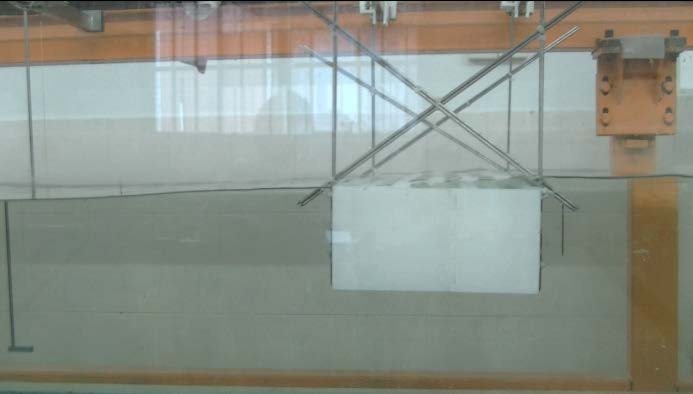
\includegraphics[width=0.6\textwidth]{48-1.png}
\caption{Wave around porous breakwater}\label{fig:48-1}
\end{figure}

\begin{figure}[!htb]
\centering
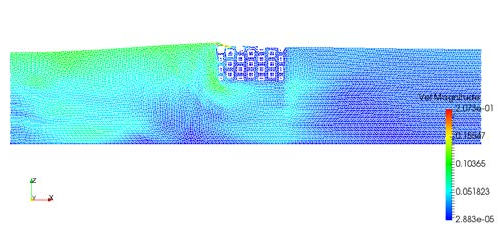
\includegraphics[width=0.65\textwidth]{48-2.png}
\caption{Velocity Field around porous breakwater (SPH)}\label{fig:48-2}
\end{figure}

\end{abstract}


%%THE END OF ABSTRACT

%\addbib

\end{document}
